Last week, we focused on hash tables and Bloom filters, which enable us to solve the \emph{dictionary problem}:
\begin{framed}
    Given a dataset $S$, subset of a very large ``universe'' $\cX$, how do we quickly check if a new element $x\in\cX$ is in the dataset?
\end{framed}
This week, we will focus on a different, but related question, which can be seen as a ``relaxed'' version of the dictionary problem. Namely, we will not ask whether a query $x$ is \emph{in} the dataset, but instead we will ask to return a point $y\in S$ that is \emph{close} to $x$~--~ideally, the closest. You can see the applications of this question: (1)~given a noisy version $x$ of an image, find the closest picture stored in the dataset (i.e., a ``denoised'' version of $x$); (2)~given a point in a high-dimensional space, cluster it by finding a close center; (3)~given an assignment submitted this semester, find the most similar in the database of assignments from previous years\dots{} those are only a few examples. 

To even start, we need to define what ``close'' means: that is, we need a notion of \emph{distance} between elements of the universe $\cX$. This can be weakened a little, but here we will assume $\cX$ is a metric space, and comes with a metric\footnote{That is, $\dist{}{}$ is non-negative,
reflexive:
\[
\dist{x}{y} = 0 \Leftrightarrow x=y
\]
symmetric:
\[
\dist{x}{y} = \dist{y}{x},
\]
and satisfies the triangle inequality:
\[
\dist{x}{y} \leq \dist{x}{z}+\dist{z}{y}
\]
for all $x,y,z\in\cX$.
}
\[
\operatorname{dist}\colon \cX\times\cX \to \R_+\,.
\]
To give an example, think of a few metrics you most likely know or have encountered before:
\begin{enumerate}
    \item The \emph{Manhattan distance} on $\cX=\R^\dims$ (a.k.a. the $\lp[1]$ distance, or taxicab distance): $\dist{x}{y} = \sum_{i=1}^\dims \abs{x_i-y_i} = \normone{x-y}$
    \item The \emph{Euclidean distance} on $\cX=\R^\dims$ (a.k.a. the $\lp[2]$ distance): $\dist{x}{y} = \sqrt{\sum_{i=1}^\dims (x_i-y_i)^2} = \normtwo{x-y}$
    \item The \emph{Hamming distance} on $\cX=\bool^\dims$: $\dist{x}{y} = \sum_{i=1}^\dims \indicSet{x_i \neq y_i}$
\end{enumerate}
Any meaningful others?

With this in hand, we can define the problem we want to solve, the \emph{Nearest Neighbour Problem:}\marginnote{Nearest Neighbour (NN)}
\begin{framed}
    Given a dataset $S$, subset of a very large metric space $(\cX,\operatorname{dist})$, how to, given a new element $x\in\cX$, output an element $y\in S$ that minimises $\dist{x}{y}$?
\end{framed}
As before, we will let $\ns=|S|$ denote the current size of the dataset (which can change as we insert or remove elements), but instead of denoting by $\green{m}$ the size of the universe $\cX$, we will instead focus on high-dimensional universes such as $\bool^\dims$ or $\R^\dims$, and denote by $\dims$ the \emph{dimension} of the universe.\marginnote{So, for $\cX = \bool^\dims$, we have $\green{m}=2^\dims$. But for $\cX=\R^\dims$, $\green{m}=\infty$.}

%%%%%%%%%%%%%%%%%%%%%%%%%%%%%%%%%%%%%%%%%%%%%%%%%%%%%%%%%%%%%%%%%%%%%%%%%%
\begin{figure}\centering


\tikzset{every picture/.style={line width=0.75pt}} %set default line width to 0.75pt        

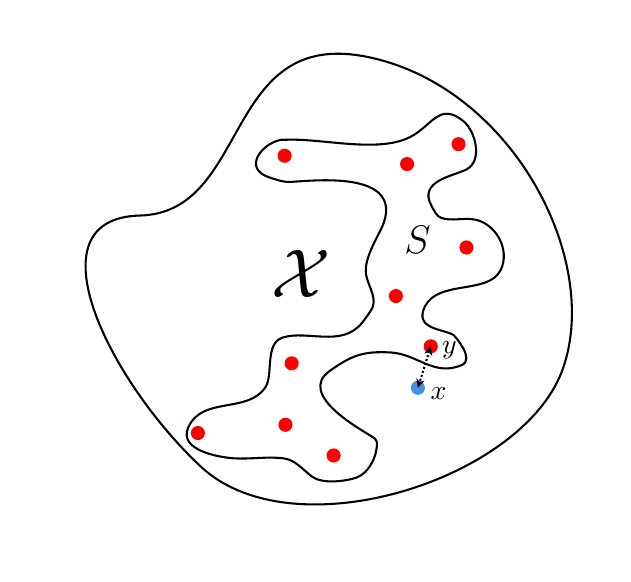
\begin{tikzpicture}[x=0.75pt,y=0.75pt,yscale=-0.8,xscale=0.8]
%uncomment if require: \path (0,300); %set diagram left start at 0, and has height of 300

%Shape: Regular Polygon [id:dp1730294945835068] 
\draw   (182.32,15.52) .. controls (268.72,32.31) and (324.31,135.62) .. (301.3,202.88) .. controls (278.28,270.15) and (138.47,314.59) .. (82.84,262.29) .. controls (27.2,209.99) and (-20.63,112.91) .. (46.25,111.25) .. controls (113.13,109.59) and (95.91,-1.27) .. (182.32,15.52) -- cycle ;
%Shape: Circle [id:dp299435924550042] 
\draw  [draw opacity=0][fill={rgb, 255:red, 255; green, 0; blue, 0 }  ,fill opacity=1 ] (196.25,159.75) .. controls (196.25,157.4) and (198.15,155.5) .. (200.5,155.5) .. controls (202.85,155.5) and (204.75,157.4) .. (204.75,159.75) .. controls (204.75,162.1) and (202.85,164) .. (200.5,164) .. controls (198.15,164) and (196.25,162.1) .. (196.25,159.75) -- cycle ;
%Shape: Circle [id:dp10120548228152837] 
\draw  [draw opacity=0][fill={rgb, 255:red, 255; green, 0; blue, 0 }  ,fill opacity=1 ] (234,68.25) .. controls (234,65.9) and (235.9,64) .. (238.25,64) .. controls (240.6,64) and (242.5,65.9) .. (242.5,68.25) .. controls (242.5,70.6) and (240.6,72.5) .. (238.25,72.5) .. controls (235.9,72.5) and (234,70.6) .. (234,68.25) -- cycle ;
%Shape: Circle [id:dp39541171931238484] 
\draw  [draw opacity=0][fill={rgb, 255:red, 255; green, 0; blue, 0 }  ,fill opacity=1 ] (203,80.25) .. controls (203,77.9) and (204.9,76) .. (207.25,76) .. controls (209.6,76) and (211.5,77.9) .. (211.5,80.25) .. controls (211.5,82.6) and (209.6,84.5) .. (207.25,84.5) .. controls (204.9,84.5) and (203,82.6) .. (203,80.25) -- cycle ;
%Shape: Circle [id:dp27264118237789015] 
\draw  [draw opacity=0][fill={rgb, 255:red, 255; green, 0; blue, 0 }  ,fill opacity=1 ] (217.25,190) .. controls (217.25,187.65) and (219.15,185.75) .. (221.5,185.75) .. controls (223.85,185.75) and (225.75,187.65) .. (225.75,190) .. controls (225.75,192.35) and (223.85,194.25) .. (221.5,194.25) .. controls (219.15,194.25) and (217.25,192.35) .. (217.25,190) -- cycle ;
%Shape: Circle [id:dp045119036480104846] 
\draw  [draw opacity=0][fill={rgb, 255:red, 255; green, 0; blue, 0 }  ,fill opacity=1 ] (77,242.25) .. controls (77,239.9) and (78.9,238) .. (81.25,238) .. controls (83.6,238) and (85.5,239.9) .. (85.5,242.25) .. controls (85.5,244.6) and (83.6,246.5) .. (81.25,246.5) .. controls (78.9,246.5) and (77,244.6) .. (77,242.25) -- cycle ;
%Shape: Circle [id:dp3583415724964084] 
\draw  [draw opacity=0][fill={rgb, 255:red, 255; green, 0; blue, 0 }  ,fill opacity=1 ] (158.75,255.75) .. controls (158.75,253.4) and (160.65,251.5) .. (163,251.5) .. controls (165.35,251.5) and (167.25,253.4) .. (167.25,255.75) .. controls (167.25,258.1) and (165.35,260) .. (163,260) .. controls (160.65,260) and (158.75,258.1) .. (158.75,255.75) -- cycle ;
%Shape: Circle [id:dp15906047769438314] 
\draw  [draw opacity=0][fill={rgb, 255:red, 255; green, 0; blue, 0 }  ,fill opacity=1 ] (133.5,200.25) .. controls (133.5,197.9) and (135.4,196) .. (137.75,196) .. controls (140.1,196) and (142,197.9) .. (142,200.25) .. controls (142,202.6) and (140.1,204.5) .. (137.75,204.5) .. controls (135.4,204.5) and (133.5,202.6) .. (133.5,200.25) -- cycle ;
%Shape: Circle [id:dp8324931679193618] 
\draw  [draw opacity=0][fill={rgb, 255:red, 255; green, 0; blue, 0 }  ,fill opacity=1 ] (129.25,75.25) .. controls (129.25,72.9) and (131.15,71) .. (133.5,71) .. controls (135.85,71) and (137.75,72.9) .. (137.75,75.25) .. controls (137.75,77.6) and (135.85,79.5) .. (133.5,79.5) .. controls (131.15,79.5) and (129.25,77.6) .. (129.25,75.25) -- cycle ;
%Shape: Circle [id:dp9687456268592909] 
\draw  [draw opacity=0][fill={rgb, 255:red, 74; green, 144; blue, 226 }  ,fill opacity=1 ] (209.5,215) .. controls (209.5,212.65) and (211.4,210.75) .. (213.75,210.75) .. controls (216.1,210.75) and (218,212.65) .. (218,215) .. controls (218,217.35) and (216.1,219.25) .. (213.75,219.25) .. controls (211.4,219.25) and (209.5,217.35) .. (209.5,215) -- cycle ;
%Shape: Circle [id:dp5806999822076053] 
\draw  [draw opacity=0][fill={rgb, 255:red, 255; green, 0; blue, 0 }  ,fill opacity=1 ] (238.75,130.5) .. controls (238.75,128.15) and (240.65,126.25) .. (243,126.25) .. controls (245.35,126.25) and (247.25,128.15) .. (247.25,130.5) .. controls (247.25,132.85) and (245.35,134.75) .. (243,134.75) .. controls (240.65,134.75) and (238.75,132.85) .. (238.75,130.5) -- cycle ;
%Shape: Free Drawing [id:dp0016405510888782837] 
\draw  [line width=0.75] [line join = round][line cap = round] (132.5,65.5) .. controls (120.64,66.63) and (107.3,82.71) .. (124.25,88.25) .. controls (127.77,89.4) and (131.31,90.77) .. (135,91) .. controls (142.47,91.46) and (204.55,81.59) .. (193.25,115.5) .. controls (191.11,121.93) and (181.01,136.28) .. (182.5,146.5) .. controls (183.45,153) and (188.5,159.42) .. (186.75,165.75) .. controls (186.04,168.31) and (180.74,175.09) .. (180,176) .. controls (167.78,190.94) and (146.96,180) .. (132.25,184.75) .. controls (121.35,188.27) and (126.79,207.08) .. (122,214.5) .. controls (111.51,230.75) and (84.05,219.84) .. (75.5,238.75) .. controls (69.18,252.74) and (94.12,256.55) .. (100.5,257.25) .. controls (111.27,258.42) and (122.25,256.12) .. (133,257.5) .. controls (140.19,258.43) and (144.71,264.63) .. (150,268.5) .. controls (156.26,273.08) and (169.72,271.29) .. (176.25,269.25) .. controls (184.31,266.73) and (189.79,255.28) .. (189,247.5) .. controls (188.86,246.15) and (187.37,245.27) .. (186.25,244.5) .. controls (180.98,240.88) and (140.1,219.28) .. (160.75,204.75) .. controls (173.61,195.7) and (180.68,192.66) .. (197.75,193.75) .. controls (213.53,194.76) and (223.66,208.48) .. (240.25,201.25) .. controls (248.2,197.78) and (236.02,183.77) .. (235.25,183.25) .. controls (229.68,179.5) and (211.02,179.96) .. (218,166) .. controls (226.06,149.87) and (256.01,158.93) .. (263.5,144.25) .. controls (269.77,131.96) and (260.54,115.32) .. (247,113.5) .. controls (240.72,112.65) and (234.04,114.68) .. (228,112.75) .. controls (225.01,111.79) and (223.52,108.24) .. (222,105.5) .. controls (213.51,90.21) and (235.59,87.42) .. (243,83.5) .. controls (253.03,78.2) and (248.46,60.44) .. (241.25,54.5) .. controls (226.63,42.46) and (222.34,57.27) .. (209,64) .. controls (188.84,74.17) and (154.17,63.97) .. (131.75,65.75) ;
%Straight Lines [id:da4336864096758598] 
\draw [line width=0.75]  [dash pattern={on 0.75pt off 0.75pt}]  (220.61,192.87) -- (218.24,200.51) -- (217.01,204.49) -- (214.64,212.13) ;
\draw [shift={(213.75,215)}, rotate = 287.22] [fill={rgb, 255:red, 0; green, 0; blue, 0 }  ][line width=0.08]  [draw opacity=0] (5.36,-2.57) -- (0,0) -- (5.36,2.57) -- (3.56,0) -- cycle    ;
\draw [shift={(221.5,190)}, rotate = 107.22] [fill={rgb, 255:red, 0; green, 0; blue, 0 }  ][line width=0.08]  [draw opacity=0] (5.36,-2.57) -- (0,0) -- (5.36,2.57) -- (3.56,0) -- cycle    ;
%Shape: Circle [id:dp774603378892477] 
\draw  [draw opacity=0][fill={rgb, 255:red, 255; green, 0; blue, 0 }  ,fill opacity=1 ] (129.75,237.25) .. controls (129.75,234.9) and (131.65,233) .. (134,233) .. controls (136.35,233) and (138.25,234.9) .. (138.25,237.25) .. controls (138.25,239.6) and (136.35,241.5) .. (134,241.5) .. controls (131.65,241.5) and (129.75,239.6) .. (129.75,237.25) -- cycle ;

% Text Node
\draw (124,130.4) node [anchor=north west][inner sep=0.75pt]  [font=\Huge]  {$\mathcal{X}$};
% Text Node
\draw (219.5,213.15) node [anchor=north west][inner sep=0.75pt]    {$x$};
% Text Node
\draw (226.5,185) node [anchor=north west][inner sep=0.75pt]    {$y$};
% Text Node
\draw (203.75,115.9) node [anchor=north west][inner sep=0.75pt]  [font=\Large]  {$S$};


\end{tikzpicture}

\end{figure}
%%%%%%%%%%%%%%%%%%%%%%%%%%%%%%%%%%%%%%%%%%%%%%%%%%%%%%%%%%%%%%%%%%%%%%%%%%

We will also for simplicity restrict ourselves to the \emph{offline} setting, where the dataset $S$ is not changing over time: instead, we are given all $\ns$ elements of $S$ at once, and can spend some time preprocessing them to create our data structure. We then only need to support the \textsc{Query} operation:
\begin{framed}
$\textsc{Query}(x)$: given an element $x\in \cX$, return an element $y\in S$ minimising $\dist{x}{y}$, that is,
$
    \dist{x}{y} = \min_{y'\in S} \dist{x}{y'}\,.
$
\end{framed}
The two main complexity measures we will seek to minimise for our data structure are:
\begin{itemize}
    \item\emph{Space complexity:} we would like our data\marginnote{Here $\dims$ takes the role of $\log\green{m}$ from the previous lecture. Can you see why?} structure to take as little space as possible, ideally $O(\ns\dims)$;
    \item\emph{Query time:} we want queries to be \emph{fast}, ideally in time \emph{sublinear in $\ns$} (and ``reasonable'' in $\dims$). For instance, $\poly(\dims)\cdot O(\ns^{0.99})$ would not be bad.
\end{itemize}
\noindent (if possible, we will also try to keep the \emph{preprocessing time} under control too, which is the time complexity of creating the data structure from the $\ns$ elements of $S$). The rationale for seeking $o(\ns)$, reasonable-in-$\dims$ query time is because while we think of the regime where the data is high-dimensional ($\dims \gg 1$), we also focus on the regime where the dataset is \emph{huge}: $\ns \gg \dims$. As a rule of thumb, you should keep in mind\marginnote{``Why?'' Note that for the case of $\cX=\bool^\dims$ for instance, $\ns$ can never be larger than $2^\dims$. And (peeking ahead), we will see the JL lemma, which in some sense guarantees that even in Euclidean space, $\dims$ can be ``made'' as small as $O(\log\ns)$.}
\[
1 \ll \dims \ll \ns \ll 2^\dims
\]
In what follows, we will also assume that we can compute distances efficiently: specifically, that $\dist{x}{y}$ can be computed in time $O(\dims)$ for any two $x,y\in\cX$; and that storing an element of $\cX$ takes space $O(\dims)$.\marginnote{Let's not get into the details of how to actually store a value $x\in\R^\dims$ on a computer.}

\paragraph{Baseline.} So, what can we do? The good news is that we can relatively easily achieve one of the two requirements. Namely:
\begin{itemize}
    \item There is a (deterministic) data structure for the Nearest Neighbour problem using space $O(\ns\dims)$, and query time $O(\ns\dims)$;
    \item There is a (deterministic) data structure for the Nearest Neighbour problem using space $O(2^\dims)$, and query time $O(2^\dims)$.\marginnote{We will see them in the tutorial.}
\end{itemize}
The bad news is that this is essentially all that we know. That is, \emph{every} data structure (even probabilistic) we know for Nearest Neighbour has either space or query complexity $\bigOmega{\min(2^\dims, \ns\dims)}$ in the worst case. 

\paragraph{Relax (the problem)!} Faced with this, a natural response is to shrug and give up. Another natural response, a few minutes later usually, is to try and modify the problem we were aiming to solve, to see if a weaker, ``relaxed'' variant could be enough (and easier). This is the basis for the \emph{Approximate Nearest Neighbour} question: instead of asking for a point $y^\ast\in S$ \emph{closest} to the query $x\in\cX$, we only ask for a point $y\in S$ that is \emph{not much further from $x$ than $y^\ast$}, \ie is ``good enough.''\marginnote{Approximate Nearest Neighbour (ANN)}
\begin{framed}
    Given a dataset $S$, subset of a very large metric space $(\cX,\operatorname{dist})$, how to, given a new element $x\in\cX$, output an element $y\in S$ that is within a constant factor of $\min_{y'\in S}\dist{x}{y'}$?
\end{framed}
Now, our data structure is parameterised by a value $\orange{C}>1$ (fixed at the creation of the data structure), and must support queries of this type:
\begin{framed}
\noindent$\textsc{Query}(x)$: given an element $x\in \cX$, return an element $y\in S$ sort-of-minimising $\dist{x}{y}$, that is,
$
    \dist{x}{y} \leq \orange{C}\cdot  \min_{y'\in S} \dist{x}{y'}\,.
$
\end{framed}
\noindent(If we were to set $\orange{C}=1$, then we would be back to the Nearest Neighbour problem.)
\section{Dimensionality reduction: the Johnson--Lindenstrauss lemma}
The first tool we will see is specific to Euclidean space ($\cX=\R^\dims$, $\dist{x}{y} = \normtwo{x-y}$), but has applications going beyond Approximate Nearest Neighbours: it is a \emph{dimensionality reduction technique} which gives a way to map points in $\R^\dims$ to points in $\R^{\purple{k}}$, for $\purple{k}\ll \dims$, while nearly preserving all their pairwise distances. That is, the Johnson--Lindenstrauss lemma gives an efficient, probabilistic mapping
\[
    \green{\Phi}\colon \R^\dims\to \R^{\purple{k}}
\]
where $\purple{k} = O(\log(1/\errprob)/\dst^2)$ such that, for any two fixed $x,y\in\R^\dims$, 
\[
    \normtwo{\green{\Phi}(x)-\green{\Phi}(y)} = (1\pm\dst) \normtwo{x-y}
\]
with probability at least $1-\errprob$. This seems quite magical: for instance, taking $\dst = 0.01$ and $\errprob=1/100$, this gives a mapping from the $\dims$-dimensional Euclidean space ($\dims$ is huge!) to a \emph{constant}-dimensional space which preserves the distance between any two points of your choosing, up to a factor $1.01$!

What is even better is that this $\green{\Phi}$ is not some insanely complicated, cumbersome to describe and impossible to implement random function. It is a random \emph{linear} mapping, obtained by just picking a random matrix $\green{M}\in\R^{\purple{k}\times\dims}$ with independent random Gaussian coefficients, and setting $\green{\Phi}(x) = \green{M}x$.~\cite{JohnsonL84}\footnote{Even, even better: subsequent work has shown how to replace ``random Gaussian coefficients'' by even simpler random coefficients (\eg in $\{-1,0,1\}$ or $\{-1,1\}$, then scaled) while preserving the same guarantees.}
\begin{theorem}[Distributional JL Lemma]
\label{theo:distr:jl}
    Fix any $\dst, \errprob\in(0,1/2)$, and set 
    \[
    \purple{k} = \bigTheta{\frac{\log(1/\errprob)}{\dst^2}}\,.
    \]
    Consider the random matrix $\green{M}\in\R^{\purple{k}\times\dims}$ obtained by drawing each entry $\green{M}_{ij}$ independently from the Gaussian distribution $\cN(0,1/\purple{k})$. Then, for any fixed $u\in \R^\dims$, we have
    \[
        \probaDistrOf{\green{M}}{(1-\dst)\normtwo{u}\leq \normtwo{\green{M}u} \leq (1+\dst)\normtwo{u}} \geq 1-\errprob\,.
    \]
\end{theorem}
We will not prove the theorem in this class, but a few remarks are in order: first, $\green{M}$ can be created in time $O(\purple{k}\dims)$ time (assuming sampling from $\cN(0,1)$ in constant time). Second, for any $x\in\R^\dims$ the projection $\green{M}x$ can be computed in time $O(\purple{k}\dims)$ as well.\footnote{There are some improvements, such as the \emph{Fast JL Transform}, to do this even faster.} Third, and this is quite important for us, this implies the following corollary, which we \emph{will} prove and is what is commonly known as ``the JL Lemma.''
\begin{corollary}[JL Lemma]
    \label{coro:jl}
    Fix any $\dst\in(0,1/2)$ and $\ns \geq 2$, and set
    \[
    \purple{k} = \bigTheta{\frac{\log \ns}{\dst^2}}\,.
    \]
    Consider the random matrix $\green{M}\in\R^{\purple{k}\times\dims}$ defined in~\cref{theo:distr:jl}. Then, for any fixed set $T\subseteq \R^\dims$ of $\ns$ elements, we have
    \[
        \probaDistrOf{\green{M}}{\forall x,y\in T,\; (1-\dst)\normtwo{x-y}\leq \normtwo{\green{M}x - \green{M}y} \leq (1+\dst)\normtwo{x-y}} \geq \frac{9}{10}\,.
    \]
\end{corollary}
\begin{proof}
    Invoke~\cref{theo:distr:jl} with $\errprob = \frac{1}{10\binom{\ns}{2}} = \bigTheta{\frac{1}{\ns^2}}$. Take a union bound over all $\binom{\ns}{2}$ pairs of distinct $x,y\in T$, applying the theorem to $u \eqdef x-y$.
\end{proof}
What this corollary promises us is that, up to a small distortion in the $\binom{\ns}{2}$ pairwise Euclidean distances of our elements, we can replace our $\dims$-dimensional Euclidean space by a much more manageable $O(\log\ns)$-dimensional Euclidean space, losing essentially nothing in the process. 

\paragraph{Application to ANN.} We can use the JL Lemma to get a somewhat non-trivial improvement over our ``baseline for Nearest Neighbour'' in the case of Euclidean space, for \emph{Approximate} Nearest Neighbour problem. Specifically, apply~\cref{coro:jl} with $\ns+1$ and small $\dst>0$ of our choosing, and get the conclusion for the set $T=S\cup \{x\} \subseteq \R^\dims$ (which is fixed, even though we do not know the query $x$ in advance). This allows us can solve the ANN problem, using the baseline approach but in $\R^{\purple{k}}$, no longer $\R^\dims$:
\begin{lemma}
For every $\dst \in(0,1/2$, there is a (probabilistic) data structure for the Approximate Nearest Neighbour problem with $\orange{C}=1+\dst$, using space $O(\frac{\ns\log\ns}{\dst^2})$, and query time $O(\frac{\ns\log\ns}{\dst^2})$, where the output to each query is correct with probability at least $9/10$.
\end{lemma}
This is not getting all the way there (we still have a near-linear dependence on $\ns$ in the query time!), but it is \emph{better.}

\section{Locality-Sensitive Hashing}
In view of what we have seen about hashing, another appealing idea would be to design some type of (family of) hash function $h\colon \cX\to\cY$ which somehow ``preserves distances'': if two elements $x,x'$ are close, then are hashed into nearby buckets, and if they are far $h$ sends them into very different buckets. In a sense, this is what the JL Lemma does for Euclidean distance: can we generalise this to other notions of distances than $\lp[2]$, and have a better control on the size ($\approx$ dimension) of the hashing space $\cY$?

\emph{Locality-Sensitivity Hashing} does exactly that, or, at least, sort of. It was introduced, for the case of Hamming distance, in an influential paper by Gionis, Indyk, and Motwani~\cite{GionisIM99}: here is the formal definition.
\begin{definition}
    Let $0\leq q< p\leq 1$, $r>0$, $\orange{C}>1$, and $(\cX,\operatorname{dist})$ be a metric space. Then a family of functions $\green{\mathcal{H}}$ from $\cX$ to $\cY$ is a \emph{$(r,\orange{C}, p,q)$-Locality Sensitive Hash family} (LSH) if, for every $x,x'\in\cX$,
    \begin{itemize}
        \item If $\dist{x}{x'} \leq r$, then $\probaDistrOf{h\sim \green{\mathcal{H}}}{h(x)=h(x')} \geq p$;
        \item If $\dist{x}{x'} \geq \orange{C}r$, then $\probaDistrOf{h\sim \green{\mathcal{H}}}{h(x)=h(x')} \leq q$;
    \end{itemize}
    and we say $\rho \eqdef \frac{\log(1/p)}{\log(1/q)} < 1$ is the \emph{sensitivity parameter} of $\green{\mathcal{H}}$.
\end{definition}
%%%%%%%%%%%%%%%%%%%%%%%%%%%%%%%%%%%%%%%%%%%%%%%%%%%%%%%%%%%%%

\begin{figure}
\tikzset{every picture/.style={line width=0.75pt}} %set default line width to 0.75pt        

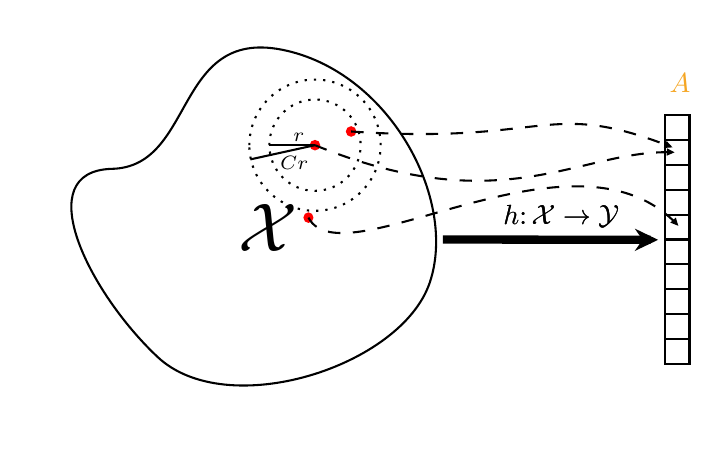
\begin{tikzpicture}[x=0.75pt,y=0.75pt,yscale=-0.6,xscale=0.6]
%uncomment if require: \path (0,300); %set diagram left start at 0, and has height of 300

%Shape: Regular Polygon [id:dp5892453846061058] 
\draw   (200.32,23.52) .. controls (286.72,40.31) and (342.31,143.62) .. (319.3,210.88) .. controls (296.28,278.15) and (156.47,322.59) .. (100.84,270.29) .. controls (45.2,217.99) and (-2.63,120.91) .. (64.25,119.25) .. controls (131.13,117.59) and (113.91,6.73) .. (200.32,23.52) -- cycle ;
%Straight Lines [id:da5940227274966229] 
\draw [line width=3]    (330,176) -- (496.75,176.24) ;
\draw [shift={(502.75,176.25)}, rotate = 180.08] [fill={rgb, 255:red, 0; green, 0; blue, 0 }  ][line width=0.08]  [draw opacity=0] (18.75,-9.01) -- (0,0) -- (18.75,9.01) -- (12.45,0) -- cycle    ;
%Shape: Grid [id:dp5884380060790032] 
\draw  [draw opacity=0] (508,76) -- (528,76) -- (528,276) -- (508,276) -- cycle ; \draw    ; \draw   (508,96) -- (528,96)(508,116) -- (528,116)(508,136) -- (528,136)(508,156) -- (528,156)(508,176) -- (528,176)(508,196) -- (528,196)(508,216) -- (528,216)(508,236) -- (528,236)(508,256) -- (528,256) ; \draw   (508,76) -- (528,76) -- (528,276) -- (508,276) -- cycle ;
%Shape: Circle [id:dp7080915007017408] 
\draw  [draw opacity=0][fill={rgb, 255:red, 255; green, 0; blue, 0 }  ,fill opacity=1 ] (252,89.25) .. controls (252,86.9) and (253.9,85) .. (256.25,85) .. controls (258.6,85) and (260.5,86.9) .. (260.5,89.25) .. controls (260.5,91.6) and (258.6,93.5) .. (256.25,93.5) .. controls (253.9,93.5) and (252,91.6) .. (252,89.25) -- cycle ;
%Curve Lines [id:da44474204475477297] 
\draw  [dash pattern={on 4.5pt off 4.5pt}]  (256.25,89.25) .. controls (415.95,100.2) and (412.13,62.13) .. (512.81,101.4) ;
\draw [shift={(514.33,102)}, rotate = 201.49] [fill={rgb, 255:red, 0; green, 0; blue, 0 }  ][line width=0.08]  [draw opacity=0] (6.25,-3) -- (0,0) -- (6.25,3) -- cycle    ;
%Shape: Circle [id:dp43426133236609155] 
\draw  [draw opacity=0][fill={rgb, 255:red, 255; green, 0; blue, 0 }  ,fill opacity=1 ] (223,100.25) .. controls (223,97.9) and (224.9,96) .. (227.25,96) .. controls (229.6,96) and (231.5,97.9) .. (231.5,100.25) .. controls (231.5,102.6) and (229.6,104.5) .. (227.25,104.5) .. controls (224.9,104.5) and (223,102.6) .. (223,100.25) -- cycle ;
%Curve Lines [id:da27933594579127596] 
\draw  [dash pattern={on 4.5pt off 4.5pt}]  (227.25,100.25) .. controls (379.22,162.13) and (439.54,103.94) .. (513.75,105.92) ;
\draw [shift={(516,106)}, rotate = 182.47] [fill={rgb, 255:red, 0; green, 0; blue, 0 }  ][line width=0.08]  [draw opacity=0] (6.25,-3) -- (0,0) -- (6.25,3) -- cycle    ;
%Shape: Circle [id:dp7752346341981025] 
\draw  [dash pattern={on 0.84pt off 2.51pt}] (190.59,100.25) .. controls (190.59,80) and (207,63.59) .. (227.25,63.59) .. controls (247.5,63.59) and (263.91,80) .. (263.91,100.25) .. controls (263.91,120.5) and (247.5,136.91) .. (227.25,136.91) .. controls (207,136.91) and (190.59,120.5) .. (190.59,100.25) -- cycle ;
%Shape: Ellipse [id:dp3531620947724323] 
\draw  [draw opacity=0][fill={rgb, 255:red, 255; green, 0; blue, 0 }  ,fill opacity=1 ] (217.92,158.42) .. controls (217.92,156.07) and (219.73,154.17) .. (221.97,154.17) .. controls (224.2,154.17) and (226.02,156.07) .. (226.02,158.42) .. controls (226.02,160.76) and (224.2,162.67) .. (221.97,162.67) .. controls (219.73,162.67) and (217.92,160.76) .. (217.92,158.42) -- cycle ;
%Curve Lines [id:da5281745957803201] 
\draw  [dash pattern={on 4.5pt off 4.5pt}]  (221.97,158.42) .. controls (249.53,210.41) and (434.47,76.35) .. (517.75,163.67) ;
\draw [shift={(519,165)}, rotate = 227.43] [fill={rgb, 255:red, 0; green, 0; blue, 0 }  ][line width=0.08]  [draw opacity=0] (6.25,-3) -- (0,0) -- (6.25,3) -- cycle    ;
%Shape: Circle [id:dp18288782111508073] 
\draw  [dash pattern={on 0.84pt off 2.51pt}] (174.55,100.28) .. controls (174.53,71.17) and (198.12,47.56) .. (227.22,47.55) .. controls (256.33,47.53) and (279.94,71.12) .. (279.95,100.22) .. controls (279.97,129.33) and (256.38,152.94) .. (227.28,152.95) .. controls (198.17,152.97) and (174.56,129.38) .. (174.55,100.28) -- cycle ;
%Straight Lines [id:da511433632598341] 
\draw    (227.25,100.25) -- (190.59,100.25) ;
%Straight Lines [id:da9934958278193481] 
\draw    (227.25,100.25) -- (175.33,111.67) ;

% Text Node
\draw (163.5,145.4) node [anchor=north west][inner sep=0.75pt]  [font=\Huge]  {$\mathcal{X}$};
% Text Node
\draw (509.5,39.9) node [anchor=north west][inner sep=0.75pt]    {$\textcolor[rgb]{0.96,0.65,0.14}{\boldsymbol{A}}$};
% Text Node
\draw (376,145.9) node [anchor=north west][inner sep=0.75pt]    {$h\colon \mathcal{X}\rightarrow \mathcal{Y}$};
% Text Node
\draw (376,145.9) node [anchor=north west][inner sep=0.75pt]    {$h\colon \mathcal{X}\rightarrow \mathcal{Y}$};
% Text Node
\draw (207.33,87.73) node [anchor=north west][inner sep=0.75pt]  [font=\scriptsize]  {$r$};
% Text Node
\draw (196.67,106.73) node [anchor=north west][inner sep=0.75pt]  [font=\scriptsize]  {$\orange{C}r$};


\end{tikzpicture}
\end{figure}
%%%%%%%%%%%%%%%%%%%%%%%%%%%%%%%%%%%%%%%%%%%%%%%%%%%%%%%%%%%%%
We will soon see the rationale behind defining this quantity $\rho$: in the meantime, as usual, a few observations:
\begin{itemize}
    \item An LSH family provides a way to control, at a given ``scale'' $r$, the collisions probabilities: sure, you \emph{will} have collisions, but points close to each other (closer than this parameter $r$) are more likely to collide than those much farther apart. This is not as strong as we would like (ideally, we would have wanted the guarantee to be true simultaneously for \emph{all} $r>0$), but this will be good enough.
    \item We would like $p$ to be as large as possible, and $q$ as small as possible: or, put differently, $\rho$ to be as large as we can achieve. This gap is what will allow us to distinguish ``far'' from ``close'' with good enough probability: if $p,q$ are almost equal, this makes our task harder.
    \item LSH families do exist (trivially): one could take $\cY=\cX$ and $\green{\mathcal{H}}$ to be the single function mapping $x$ to itself. This is not interesting at all (it does not save space, time, or anything really), but at least it shows this definition is not impossible to satisfy. What remains is to get more interesting LSH families, with small $\cY$.
\end{itemize}
As a start, we will show how to, given an LSH family for a specific scale $r>0$, solve a ```baby version'' of our Approximate Nearest Neighbour question: that is, we will give a data structure that, after preprocessing, supports the following query, for fixed values of $r>0$ and $\orange{C}>1$.
\begin{framed}
\noindent$\textsc{Query}_r(x)$: given an element $x\in \cX$, return an element $y\in S$, or $\bot$, such that:
\begin{itemize}
    \item If there exists $y^\ast\in S$ such that $\dist{x}{y^\ast} \leq r$, then, with probability at least $9/10$, $\textsc{Query}_r(x)$ returns an element $y\in S$ such that $\dist{x}{y^\ast} \leq \orange{C}\cdot r$;
    \item If $\dist{x}{y} > \orange{C}\cdot r$ for \emph{every} $y\in S$, then, with probability $1$, $\textsc{Query}_r(x)$ returns $\bot$.
    \item Otherwise, any output in $S\cup\{\bot\}$ is allowed.
\end{itemize}
\end{framed}
To solve this ``baby ANN version,'' we will use\dots hash tables. But in addition to a standard, run-of-the-mill good hashing family for the hash tables, we will also use an $(r,\orange{C}, p,q)$-LSH family, which we assume is given to us (we will later show how to design such an LSH family): in what is below, $\purple{k}$ and $\red{\ell}$ are integers, whose values we will carefully choose after analysing the guarantees of our data structure. We first need the following fact, which allows us to ``tune'' the parameters $p,q$ of an LSH family.
\begin{lemma}
    Suppose $\green{\mathcal{H}}$ from $\cX$ to $\cY$ is an $(r,\orange{C}, p,q)$-LSH family, and fix any integer $\red{\ell}\geq 1$. For any $g_1,\dots, g_{\red{\ell}}\in \green{\mathcal{H}}$, define the function $g\colon \cX\to \cY^{\red{\ell}}$ by
    \[
        g(x) = (g_1(x),\dots, g_{\red{\ell}}(x))\in \cY^{\red{\ell}}
    \]
    Then, the resulting family $\green{\mathcal{H}^{(\red{\ell})}} \eqdef \{ (g_1,\dots, g_{\red{\ell}})\colon \cX\to \cY^{\red{\ell}} \}$ is an $(r,\orange{C}, p^{\red{\ell}},q^{\red{\ell}})$-LSH family of size $|\green{\mathcal{H}}|^{\red{\ell}}$ (and as a result has the same sensitivity parameter $\rho$).
\end{lemma}
\begin{proof}
    ``Proof by writing it down.''
\end{proof}
Intuitively, this gives us some flexibility when designing our data structure:\marginnote{``What is the point of this $\red{\ell}$?''} we do not get to choose $p,q$, and would like both (1)~$p$ to be large (better chances of finding close elements, and so smaller probability of failure) \emph{and} (2)~$q$ to be small (fewer ``spurious'' collisions introduced, which will mean better query complexity in our final hash table-based data structure). This parameter $\red{\ell}$ allows us to control (2) (as $q^{\red{\ell}}$ can be made as small as we want), at the price of making (1) worse as well ($p^{\red{\ell}}$ goes down too); fortunately, we will soon introduce our other parameter $\purple{k}$ which will give us control over (1), and so we will be able to achieve both (1) \emph{and} (2) by carefully balancing $\purple{k}$ and $\red{\ell}$.\smallskip

\noindent Let us now actually describe our data structure:
\begin{framed}
\noindent For a fixed, given $r$ (and some $\orange{C}>1$), let $\green{\mathcal{H}}$ be an $(r,\orange{C}, p,q)$-LSH family. Let $g_1,\dots, g_{\purple{k}}\colon \cX\to\cY^{\red{\ell}}$ be hash functions chosen independently from $\green{\mathcal{H}}^{(\red{\ell})}$. Build $\purple{k}$ hash tables $(\orange{A}_1, h_1),\dots, (\orange{A}_{\purple{k}}, h_{\purple{k}})$ with separate chaining, where $h_1,\dots, h_{\purple{k}}\colon \cY\to\cZ$ are $\purple{k}$ independent ``standard'' hash functions from a suitable hashing family.
\begin{itemize}
\item$\textsc{Preprocess}(S)$:
            \begin{algorithmic}
                \ForAll{$x\in S$} \Comment{Insert all $\ns$ elements in all $\purple{k}$ hash tables, using their LSH hashing as keys}
                    \ForAll{$1\leq t\leq \purple{k}$}
                        \State $\orange{A}_{t}[h_t(g_t(x))].\textsc{Insert}(x)$
                    \EndFor
                \EndFor
            \end{algorithmic}

\item$\textsc{Query}_r(x)$: 
            \begin{algorithmic}
                \ForAll{$1\leq t\leq \purple{k}$}
                        \State $L_t\gets \orange{A}_t[h_t(g_t(x))]$ \Comment{List of elements of $S$ colliding with $g_t(x)$ in the $t$-th hash table}
                        \ForAll{$y\in L_t$}
                            \If{$\dist{x}{y} \leq \orange{C}\cdot r$}\label{step:lsh:checkdistance}
                                \State\Return $y$ \Comment{Found one!}
                            \EndIf
                        \EndFor
                \EndFor
                \State\Return $\bot$ \Comment{Did not find any.}
            \end{algorithmic}
\end{itemize}
\end{framed}
Note that we use both the locality-sensitive hash functions $g_t$ \emph{and}\marginnote{``Why do we use two types of hash functions?''} the ``regular'' hash function $h_t$: this is to save space, as if we only used the former we would have the ``locality sensitive'' part, but none of the good guarantees from usual hash functions (small number of hash buckets, along with small collision probability) which allowed us last lecture to argue hash tables were space-efficient. That is, we use two levels of hashing, with two different ``types'' of hash functions:
\begin{itemize}
    \item the first level uses the LSH function $g_t$ to hash elements in a ``locality-sensitive way'' (we \emph{want} close elements to collide, but far elements to go to distinct buckets): this is the main conceptual idea. However, these at-most-$\ns$ resulting elements $S'_t\eqdef \{g_t(x)\}_{x\in S}$ still live in a very big space (\ie $\cY^{\red{\ell}}$), so storing them naively would not be space-efficient; and so,
    \item the second level uses the ``usual'' hash functions $h_t$ to hash this set of ``LSH hashes'' $S'_t$ in a ``standard hash table way'' (we want as few collisions as possible), to save space.
\end{itemize}


We will establish the following guarantees for this data structure, assuming each hash function from $\green{\mathcal{H}}$ can be evaluated in time $T$ and each hash table $\orange{A}_t$ uses space $O(\ns\dims)$:\marginnote{We can improve the $O(\purple{k}\ns\dims)$ space complexity to $O(\purple{k}\ns\log\ns + \ns\dims)$, by only keeping the index of each element $x\in S$ in the data structure along with a separate array containing all of them, to look up where the $i$-th element actually is.}
\begin{theorem}
    The data structure described above for the ``baby version of ANN'' has space complexity $O(\purple{k}\ns\dims + \purple{k}\red{\ell}\dims)$, expected query complexity $O(\purple{k}\red{\ell}T+\purple{k}\ns\dims q^{\red{\ell}})$, and satisfies the correctness requirements as long as $(1-p^{\red{\ell}})^{\purple{k}} \leq \frac{1}{10}$.
\end{theorem}
\begin{proof}
    The space complexity follows from that of the $\purple{k}$ hash tables, each of which using space $O(\ns\dims)$ (we also have to account for the storage of the $\purple{k}$ ``$\red{\ell}$-fold'' LSH hash functions, which we assume can be done with $\red{\ell}\cdot O(\dims)$ bits each). 
    
    The expected query time comes from (1)~evaluating (up to) $\purple{k}$ hash functions $g_1(x),\dots, g_{\purple{k}}(x)$, for a total time $O(\purple{k}\red{\ell}T)$; (2)~for each $1\leq t\leq \purple{k}$, checking the distance to $x$ of every point in the list $L_t$ until we find one that is at distance less than $\orange{C}r$. So we only have to count the expectation number of \emph{false positives} which collide but are far, since a true positive $y$ will be a success, and causes the function to immediately stop and return $y$.  Each distance computation can be done in time $O(\dims)$, and by the LSH guarantee we have on expectation at most 
    \[
        \ns\cdot q^{\red{\ell}}
    \]
    such false positives (points $y$ such that $\dist{x}{y} \geq C\cdot r$ but with $g_t(x)=g_t(y)$); to this, we must add an additional expected $O(1)$ ``standard hash collisions,'' just from the usual guarantees of good hash tables. So that gives us expected query time at most
    \[
        O(\purple{k}\red{\ell}T) + \purple{k}\cdot \Paren{\ns\cdot q^{\red{\ell}}+O(1)} \cdot O(\dims)
        = O(\purple{k}\red{\ell}T+\purple{k}\ns\dims q^{\red{\ell}})
    \]
    assuming, for the last part, that $\ns q^{\red{\ell}} = \Omega(1)$.\footnote{In particular, there is no point in setting $\red{\ell}$ such that $\ns q^{\red{\ell}} \ll 1$, as the $O(1)$ term would then dominate.}

    For the correctness, first observe that the second item is immediate from definition of the algorithm: since Line~\ref{step:lsh:checkdistance} checks the distance is at most $\orange{C}\cdot r$, if every point in $S$ is at distance greater than $\orange{C}\cdot r$ from $x$ then the algorithm will always output $\bot$. The first item is trickier: assume there is a point $y^\ast$ such that $\dist{x}{y^\ast} \leq r$. Then the probability that \emph{none} of the $\purple{k}$ LSH hash functions ``collide'' is at most
    \[
        \probaOf{ \forall t\in[\purple{k}],\; g_t(x) \neq g_t(y^\ast) } \leq (1-p^{\red{\ell}})^{\purple{k}} \leq \frac{1}{10}\,.
    \]
    This is \emph{the} bad event: if it does not happen, then at least one of the $\purple{k}$ hash tables will map $x$ and $y^\ast$ to the same bucket, and so at least one $y$ will pass the test in Line~\ref{step:lsh:checkdistance} (at the very least, $y^\ast$ would: another $y$ might be returned earlier).
\end{proof}
This is encouraging, but we have a \emph{lot} of parameters there. \emph{How should we set $\purple{k}$ and $\red{\ell}$}?
\begin{itemize}
    \item From the second term in the expected query complexity, by setting 
    \begin{equation}
        \label{eq:lsh:setting:l}
        \red{\ell} \eqdef \frac{\log \ns}{\log(1/q)}
    \end{equation}
    we get $q^{\red{\ell}} = 1/\ns$, and so the expected query time becomes $O(\purple{k}\red{\ell}T+\purple{k}\dims)$.
    \item This gives us $p^{\red{\ell}} = 2^{-\red{\ell}\log(1/p)} = \ns^{-\rho}$,\marginnote{``A wild sensitivity parameter $\rho$ appears''} and to satisfy the correctness condition 
    \[
        (1-p^{\red{\ell}})^{\purple{k}} \leq \frac{1}{10}
    \]
    it is then sufficient (and necessary) to set\marginnote{Check it!}
    \begin{equation}
        \label{eq:lsh:setting:k}
        \purple{k} = O(n^{\rho})
    \end{equation}
\end{itemize}
This finally gives us the following (recalling that $\log\ns \ll \dims$ to simplify the query complexity):
\begin{corollary}
    With the settings of $\purple{k},\red{\ell}$ from~\cref{eq:lsh:setting:l,eq:lsh:setting:k} and assuming $q,T=\Theta(1)$, the data structure for the ``baby version of ANN'' has space complexity $O(\ns^{1+\rho}\dims)$ and expected query complexity $O(\ns^\rho\dims)$.
\end{corollary}
This is quite good: the space is only ``mildly worse'' than the necessary $\ns\dims$, and query complexity is \emph{sublinear} in $\ns$, since $\rho < 1$!\bigskip

\textbf{But}\dots this was just a ``baby'' version of our problem: this did not solve the ANN question itself! Thankfully, there is a `simple'' reduction from this version (where $r$ is ``hardcoded'') to the general case:
\begin{theorem}
    Suppose that, for every $0 < r\leq \dims$, we have a data structure for the ``baby'' version of ANN with scale parameter $r$ and parameter $\orange{C}>0$, with space complexity $S(\ns,\dims)$, expected query complexity $T(\ns,\dims)$ and probability of failure $\errprob$ per query. Then there is a data structure for ANN with parameter $2\orange{C}$, space complexity $O(S(\ns,\dims)\log^2\ns)$, expected query complexity $O(T(\ns,\dims)\log\ns)$, and probability of failure $\errprob\log\ns$ per query..
\end{theorem}
\begin{proof}
    This reduction is quite involved, and was shown in Theorem~2.9 of~\cite{HarPeledIM12}. In the tutorial, you will see a much simpler version, losing instead a logarithmic factor in the ``aspect ratio''
    \[
        \Delta \eqdef \frac{\max_{x,x'} \dist{x}{x'}}{\min_{x,x'} \dist{x}{x'}}
    \]
    using, essentially, a doubling search over $r$.
\end{proof}
At this point, we know what to do if we are \emph{given} an LSH family for the metric space $(\cX,\operatorname{dist})$ we care about~--~and the smaller the parameter $\rho$ of that LSH family is, the better the query times and space complexity we will obtain are. Which brings a very natural question:
\begin{framed}
   \noindent Are there good  LSH families for the metric spaces we care about?
\end{framed}
\noindent We will give two examples, showing that the answer is (mostly) ``yes.''
\subsection{Example: Hamming space}
The first example is that of the \emph{Hamming space of dimension $\dims$}, which, again, is just a fancy way of saying ``the universe of $\dims$-bit strings where the distance between two $x,x'\in \cX = \bool^\dims$ is the number of bits in which they differ.''

What will be the LSH family? The simplest thing one could think of: $\green{\mathcal{H}}$ will just be the set of $\dims$ functions
\[
    h_i\colon \bool^\dims\to \bool, \qquad 1\leq i\leq \dims
\]
where $h_i(x) = x_i$ just ``hashes'' a string $x$ to its $i$-bit. That's all! One can then verify that, for every $1\leq r\leq \dims$ and $\orange{C}>1$,\marginnote{If $\orange{C}r > \dims$ the guarantee is trivially true.}
    \begin{itemize}
        \item If $\dist{x}{x'} \leq r$, then $\probaDistrOf{h\sim \green{\mathcal{H}}}{h(x)=h(x')} \geq 1-\frac{r}{\dims}$;
        \item If $\dist{x}{x'} \geq \orange{C}r$, then $\probaDistrOf{h\sim \green{\mathcal{H}}}{h(x)=h(x')} \leq 1-\frac{\orange{C}r}{\dims}$;
    \end{itemize}
and so this $\green{\mathcal{H}}$ is an $(r,\orange{C}, p,q)$-LSH family for $p\eqdef 1-\frac{r}{\dims}, q\eqdef 1-\frac{\orange{C}r}{\dims}$, with size $|\green{\mathcal{H}}|=\dims$ and sensitivity
\begin{equation}
    \rho = \frac{\log\Paren{1-\frac{r}{\dims}}}{\log\Paren{1-\frac{\orange{C}r}{\dims}}} \approx \frac{1}{\orange{C}}\,.
\end{equation}
\noindent(as a side note, it has been shown that $\rho = \Theta(1/\orange{C})$ is the best one can get for the Hamming space.)
\subsection{Example: Euclidean space ($\lp[2]$ distance)}
What about the Euclidean space? Recycling is good, so we may want to use some of the ideas behind the JL Lemma to design a good LSH Family. Fortunately, this is possible: pick a random vector $\green{g}\sim\cN(0,I_{\dims})$, and set
\begin{equation}
    h_{\green{g}}(x) = \operatorname{sign}(\langle \green{g}, x \rangle) \in \{-1,1\}
\end{equation}
(that is, pick a random gaussian vector $\green{g}$, and take the sign of the inner product between $\green{g}$ and $x$). One can show\footnote{And you will in the tutorial.} that, for every $r>0$ and $\orange{C}>1$, this gives an LSH family with sensitivity parameter
\begin{equation}
    \rho \leq \frac{1}{\orange{C}}\,.
\end{equation}
Interestingly, this is not optimal! For the Euclidean space, more involved constructions are able to obtain LSH families with sensitivity parameter $\rho = O(1/\orange{C}^2)$.


%https://www.cs.princeton.edu/~hy2/teaching/fall22-cos521/notes/NNS%20&%20LSH.pdf
% https://cs368-stanford.github.io/spring2022/lectures/lec17.pdf

% Some other lecture notes:
% https://www.cs.toronto.edu/~anikolov/CSC473W20/Lectures/LSH.pdf
% https://www.cs.princeton.edu/courses/archive/fall18/cos521/Lectures/lec12.pdf
% https://cs368-stanford.github.io/spring2022/lectures/lec16.pdf
% https://cs368-stanford.github.io/spring2022/lectures/lec17.pdf (mentions the Kane-Nelson faster JL)
% https://www.cs.cmu.edu/~15451-s19/lectures/lec22-nearest-neighbor.pdf

% https://www.cs.columbia.edu/~andoni/LSH/